\section{Démarche de médecine factuelle}

\subsection{Informations scientifiques}
  
\subsubsection{Méthode}

PICO :
\begin{itemize}[label=\textbullet]
    \item Population : Patient souffrant d’un épisode dépressif résistant avec caractéristiques mixtes. 
    \item Intervention : l’ajout d’antipsychotiques au traitement antidépresseur. 
    \item Comparateur : placebo. 
    \item Outcome : obtenir une rémission des symptômes et prévenir les effets secondaires. 
\end{itemize}

Banque de données consultée : Pub Med.\\ 
Termes MeSH utilisés : «Major Depressive Disorder », «Mania» et «Antipsychotic Agents».\\
Critère pour la sélection d’article : publication dans les $5$ ans, «Free full text», «Randomized controlled trial», «Meta-analyse» et «Systematic review».\\
Date de consultation et nombre d’articles : le $07$ février $2026$, $2$ articles répondaient à ces critères. 

\subsubsection{Résultats}  

L'article choisi est le suivant, \textcite{gao2025efficacy}.
 
Les auteurs constatent une amélioration des symptômes dépressifs et maniaques avec les antipsychotiques chez les patients souffrant de MDE-MFS -- major depressive episodes with mixed features specifier. Ce traitement aurait un profil des effets secondaires bénéfiques sans risque augmenté d’effets secondaires sévères. Les stabilisateurs de l’humeur et certains antidépresseurs -- trazodone -- montreraient également une efficacité chez ces mêmes patients. Toutefois, la preuve de leur efficacité et leur sécurité étaient limitées et controversées dû au nombre restreint d’études disponibles.

\begin{figure}[H]
    \centering
    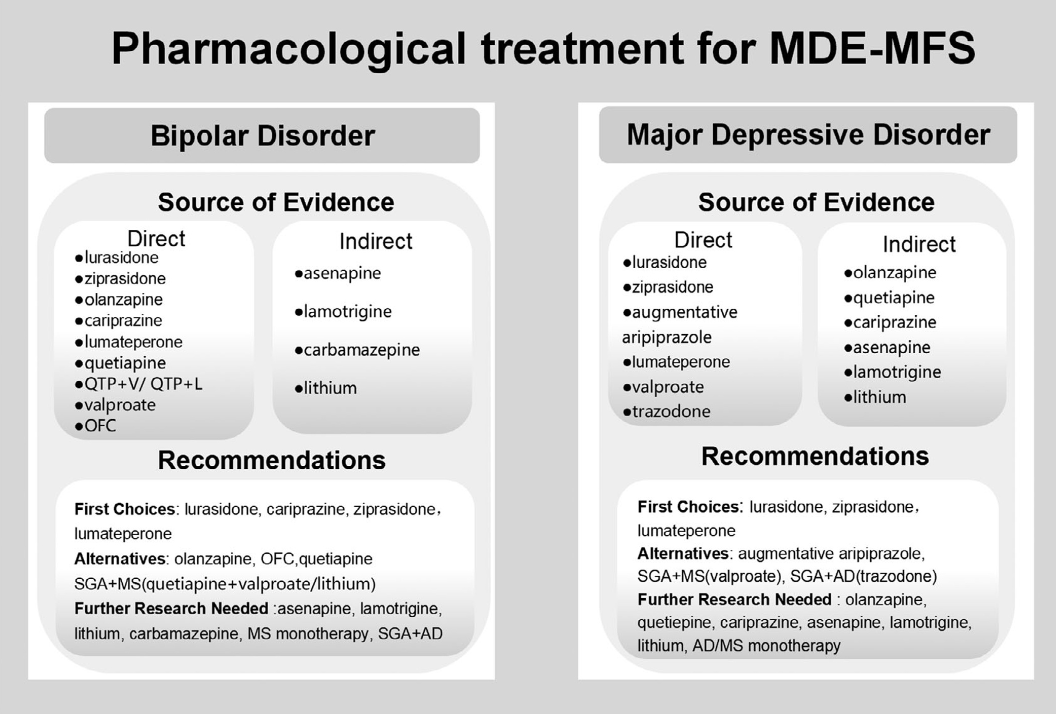
\includegraphics[width=\textwidth]{images/cas_therapeutique/resultat_etude_casM2.png}
    \caption{traitement pharmacologique pour MDE-MFS}
    \label{fig:resultat_etude_casM2}
\end{figure}

\subsubsection{Discussion}





\begin{itemize}[label=\textbullet]
    \item \textbf{Analyse critique de la méthodologie}\\
    La méthodologie de cette méta-analyse, notamment pour évaluer puis stratifier les différents articles selon leur biais, semble complète et rigoureuse tout à fait en accord avec l’EBM. Pour chaque nature d’article, différents outils adaptés ont été employés \todoH{FloraStyle}{red!30}{Cochrane tool (Higgins et al., 2011) : C'est le standard mondial ("gold standard") pour évaluer les biais dans les essais contrôlés randomisés (RCT). Il analyse précisément la randomisation et l'insu.
    Newcastle-Ottawa Scale (NOS) : C'est l'outil de référence pour les études observationnelles et les analyses post-hoc.
    ROBINS (Risk of Bias In Non-randomized Studies) : C'est l'outil le plus robuste recommandé par la collaboration Cochrane pour les études d'intervention non randomisées.
    Outils JBI (Joanna Briggs Institute) : Ils sont reconnus internationalement pour l'évaluation rigoureuse des séries de cas et des rapports de cas.}{(Cochrane pour les RCTs, NOS pour les études observationnelles, ROBINS pour les études ouvertes).}
    
    Concernant le biais de publication, il a été mesuré selon plusieurs outils, à nouveau pour argumenter et valider au mieux les résultats. Le funnel plot est cependant difficilement interprétable vu le nombre d’études sélectionnées inférieur à 10 mais le test d’Edgar avec p≥$0,05$ confirme l’absence de biais de publication significatif.
    
    L’analyse de la sensibilité via la méthode «leave-one-out» a démontré qu’une étude en particulier, l'étude de Singh et al. ($2020$) sur les adolescents, déstabilisait les résultat concernant les symptômes maniaques et donc montre un I$^2$ élevé. Afin de résoudre cette forte hétérogénéité, cette étude a été exclue. 
    
    Les méthodes utilisées pour interpréter les résultats de cette méta-analyse semblent répondre à l’EBM. Toutefois, le talon d’Achille de cette étude est le nombre d’études disponibles et leur qualité intrinsèque, en effet la majorité des articles étaient des analyses post-hoc, c’est-à-dire, des analyses qui n’avaient pas pour objet la thématique de cette méta-analyse mais dont les données ont été recueillies. Les auteurs qualifient donc cette méta-analyse de préliminaire, nécessitant par la suite des RCT prospectifs. De plus, les variations de définition de dépression avec caractéristiques mixtes sont retrouvées dans la littérature médicale ce qui complique la réalisation de la méta-analyse et peut-être biaise la sélection des patients. 
    
    \item \textbf{L'interprétation des principaux résultats}\\
    Concernant les antipsychotiques, le taux de réponse clinique est meilleur par rapport au placebo  (RR = $1.46$ [$95$\% CI: $1.31, 1.61$], p < $0.001$; NNT = $7 [95$\% CI: $5, 9$]).  Les autres outcomes primaires tels que l’évolution du \todoH{FloraStyle}{red!30}{\url{https://www.ciusss-capitalenationale.gouv.qc.ca/sites/d8/files/docs/ProfSante/Infirmier/evaluation-manie-young.pdf}}{score YMRS}, l’échelle d’évaluation de la manie de Young, montrent une nette réduction comparée au placebo (SMD = $0.35 [95\% CI: 0.53, 0.17], p < 0.001$). 
    
    Quant à l’outcome primaire de sécurité, TEM rate qui signifie le virage maniaque, n’est pas significativement différent du groupe contrôle (RR = $0.91 [95\% CI: 0.53, 1.55], p = 0.65$). Par contre, les antipsychotiques ont été associés à une recrudescence du risque d’effets secondairess classique par rapport au placebo (RR = $2.33 [95\% CI: 1.63,3.34], p < 0.001; NNH = 17 [95\% CI: 11,25$]) particulièrement pour les symptômes extrapyramidaux et le trouble de la vigilance et du sommeil.
    
    Les auteurs ont également analysé l’efficacité et la sécurité de différents types d’antipsychotiques chez les patients souffrant de d’épisodes dépressifs majeurs avec caractéristiques mixtes dans un contexte de dépression majeure. Cependant, le nombre restreint d'études disponibles pour ce profil clinique spécifique a limité les conclusions à une analyse descriptive, empêchant la réalisation d'une synthèse quantitative formelle. Malgré cette limite, les données révèlent une efficacité supérieure des antipsychotiques sur le placebo pour stabiliser les deux pôles de la pathologie. La lurasidone a notamment montré un taux de réponse supérieur au placebo ($64.8\% $versus $30.0\%, p < 0.001$), avec une amélioration des symptômes maniaques confirmée à long terme.  Sur le plan de la sécurité, aucune augmentation significative du risque de virage maniaque (taux de TEM) ou de symptômes extrapyramidaux (EPS) n'a été observée par rapport au placebo, les effets indésirables courants comme la somnolence ou les nausées restant généralement modérés et tolérables.
    
    Toujours en reprenant cette population précise, une étude a montré une amélioration significative des symptômes dépressifs grâce aux stabilisateurs de l’humeur (valproate) à dose moyenne chez $18/22$ patients. Lors du suivi, certains ont rapporté des effets secondaires et un tiers de ces personnes ont arrêté le traitement pour cette raison. Deux études rétrospectives indiquent enfin que la trazodone pourrait réduire efficacement l’agitation et les symptômes mixtes avec un profil de sécurité rassurant, bien que l’absence de groupe contrôle impose de considérer ces résultats comme préliminaires.
\end{itemize}
 
\subsubsection{Conclusion} 
 
Cet article confirme les guidelines et appuie la sécurité et l’efficacité des antipsychotiques, régulateur de l’humeur et de certains antidépresseurs dans ce contexte de MDD avec MDE-MFS. Toutefois, il faut garder à l’esprit les limites de cette méta-analyse notamment le nombre limité d’études disponibles et que les auteurs ont décidé d’inclure des analyses post-hoc. 
 
\subsection{Contextualisation}
La patiente, au cours de sa prise en charge, a souffert de nombreux effets secondaires. Certains s’associent à des pathologies déjà présentent, notamment les troubles de transites qui s’additionnent aux diarrhées chroniques idiopathiques. 

En pratique, vu les traitements antérieurs et leur tolérance chez la patiente, plusieurs molécules étaient éliminées dont la quétiapine, le valproate. Un régulateur de l’humeur était à envisager compte tenu des caractéristiques mixtes de sa dépression. L'olanzapine semblait donc une molécule de choix pour associé à la paroxetine vu son efficacité prouvée sur ce type de diagnostic. Cependant, l'hypercholestérolémie objectivée par le bilan biologique constitue un paramètre de vigilance majeur, car l'olanzapine est étroitement associée à un risque accru de dyslipidémie et de syndrome métabolique.

Si l’on suit les recommandations de la méta-analyse la lurasidone pourrait être également une alternative vu son profil d’efficacité et de tolérance dans la population MDD avec MDE-MFS. La trazodone pourrait également apporter des effets positifs chez la patiente, tout en s’assurant de la bonne tolérance de la patiente.

Il est important de noter que la patiente est compliante et vu son éducation thérapeutique et ses croyances, avoir un traitement comprenant plusieurs comprimés quotidiens ne représente pas un obstacle à la prise en charge.

La prise en charge de la patiente doit prendre en considération la sphère sociale. En particulier, le déclencheur principal de cette hospitalisation a été son fils. Par conséquence, la situation ne sera pas résolue tant que le fils habitera avec la patiente. C’est pourquoi une cure psychothérapeutique stationnaire a, en partie, été mise en place afin de solutionner temporairement le problème social et évidemment pour traiter la patiente au niveau psychologique. Le traitement médicamenteux a aussi son rôle à jouer pour stabiliser la patiente à court terme lorsque le travail psychologique et social se résout à long terme. 

\subsection{Intégration}
La littérature médicale permet de guider le praticien. Bien sûr les guidelines ont leur place dans la prise de décision du médecin. Cependant, la patiente doit être au centre des soins et elle n’est pas égale à la population générale. Il faut donc adapter sa prise en charge à la personne qui est souffre de la pathologie en question et l’adapter à son contexte social et familial. Dans ce cas, la patiente a besoin de prise en charge psychologique et sociale qui ne peuvent pas se résoudre rapidement. La décision d’un traitement médicamenteux est justifiée vu les effets bénéfiques sur les symptômes de la patiente.

Concernant le choix de la molécule, sa tolérance particulière aux molécules, marquée par une susceptibilité allergique cutanée, devient ici le principal guide du choix thérapeutique, primant sur les recommandations générales de première intention ou celles avancées par la méta-analyse. De plus, en pratique, toutes les molécules ne sont pas disponibles au Grand-Duché du Luxembourg notamment lurasidone. Le praticien doit donc adapter sa prise en charge en fonction des limitations pratiques qui se présentent à lui.